% Created 2021-09-29 Wed 20:00
% Intended LaTeX compiler: xelatex
\documentclass[bigger]{beamer}
\usepackage{graphicx}
\usepackage{grffile}
\usepackage{longtable}
\usepackage{wrapfig}
\usepackage{rotating}
\usepackage[normalem]{ulem}
\usepackage{amsmath}
\usepackage{textcomp}
\usepackage{amssymb}
\usepackage{capt-of}
\usepackage{hyperref}
\usepackage{pifont}
\usepackage{verbatim}
\makeatletter
\def\verbatim@font{\scriptsize\ttfamily}
\makeatother
\logo{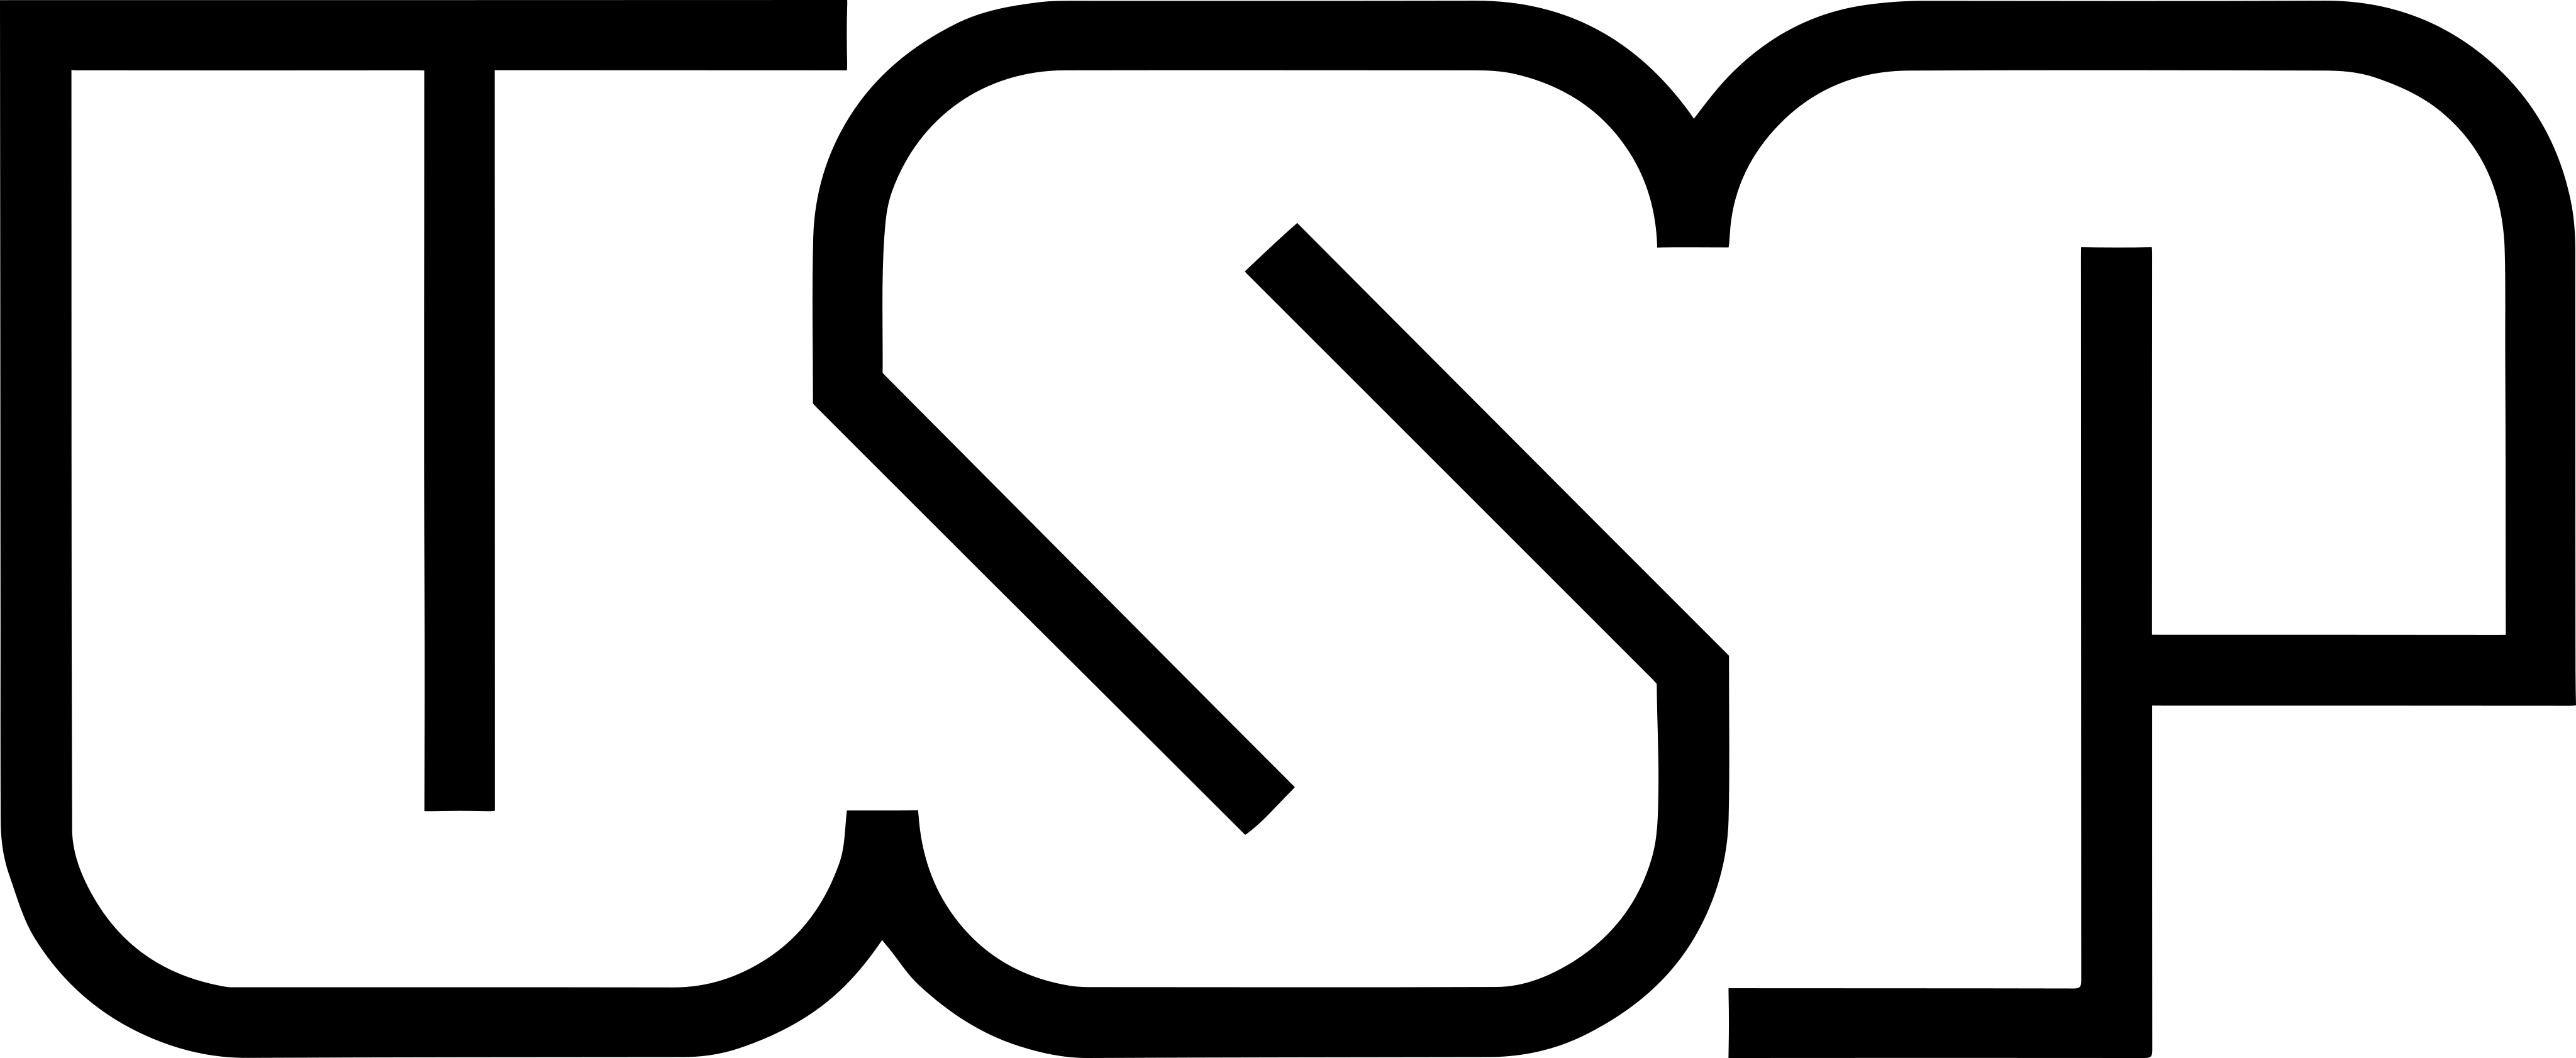
\includegraphics[height=0.5cm]{../Apresetacoes/Apres1/img/usp-logo-1}}
\AtBeginSubsection[]{\begin{frame}\frametitle{Table of Contents}\tableofcontents[currentsection,currentsubsection]\end{frame}}
\usepackage{tikz}
\usetikzlibrary{arrows.meta}
\usetikzlibrary{positioning}
\usepackage{tcolorbox}
\tcbuselibrary{skins}
\usepackage{minted}
\usemintedstyle{vim} %lovelace
\usepackage{listings}
\newenvironment{modern-quote}{\begin{itemize}}{\end{itemize}}
\tcolorboxenvironment{modern-quote}{blanker,before skip=6pt,after skip=6pt, borderline west={3mm}{0pt}{black!90!white}, colframe=black!90!white}
\newenvironment{modern-quote-env}{\begin{itemize}}{\end{itemize}}
\tcolorboxenvironment{modern-quote-env}{before skip=6pt,after skip=6pt, borderline west={3mm}{0pt}{black!10!white}, colframe=black!50!white}
{\usebackgroundtemplate{
\includegraphics[height=\paperheight]{../Apresetacoes/Apres1/img/TP-yellow-34.jpg}}
\setbeamertemplate{frame footer}{SEMEF VIII}
\usetheme{metropolis}
\usecolortheme{magpie}
\date{  Universidade de São Paulo - DEMAR}
\title{O \LaTeX{}, uma roupagem metropolitana}
\author[Branquinho]{\textbf{Pedro Gomes Branquinho \\ \text{\scriptsize{pedro.branquinho@usp.br}}}}
\date[EEL-USP]{\textbf{\scriptsize{Mini-curso de \LaTeX} \\ Universidade de São Paulo - DEMAR}}
\metroset{block=fill, background=dark}
\setbeamertemplate{itemize item}{\ding{166}}
\setbeamercolor{item projected}{bg=magenta!90!black,fg=white}
\setbeamertemplate{enumerate item}[circle]
\setbeamerfont{block title}{size={\centering}}
\setbeamercolor{block title}{bg=black!30!white,fg=white}
\setbeamertemplate{sections/subsections in toc}[square]
\setbeamerfont{section in toc}{size=\large,series=\bfseries}
\setbeamercolor{section in toc}{bg=black, fg=white!80!yellow}
\hypersetup{
 pdfauthor={},
 pdftitle={O \LaTeX{}, uma roupagem metropolitana},
 pdfkeywords={},
 pdfsubject={},
 pdfcreator={Emacs 27.2 (Org mode 9.4.4)}, 
 pdflang={Portuguese}}
\begin{document}

\maketitle
\begin{frame}{Outline}
\tableofcontents
\end{frame}

{\usebackgroundtemplate{\includegraphics[height=\paperheight]{../Apresetacoes/Apres1/img/yellow-30.jpg}}

\section{Codigo fonte}
\label{sec:org0d36e7c}
\begin{frame}[label={sec:org594b747}]{Repositorio}
Podemos acessar o codigo fonte da instalaçao por esse link:
\textbf{https://github.com/matze/mtheme/tree/master/source}

\transdissolve
\end{frame}
\begin{frame}[label={sec:org273d7c6},fragile]{Compile o .sty localmente}
 \begin{block}{Passos para compilar o \alert{estilo} localmente}
\fvset{listparameters=\setlength{\topsep}{0pt}\setlength{\partopsep}{0pt}}
\begin{enumerate}[<1->]
\item \small{Clone o repositorio}
\item \small{Entre no diretorio}
\end{enumerate}
\begin{minted}[frame=lines,fontsize=\scriptsize,linenos=true]{shell}
git clone https://github.com/matze/mtheme

cd mtheme
\end{minted}

\begin{enumerate}[<2->]
\item \small Compile, e instale, com \alert{make}, os arquivos sty;
\item \small{Faça o ecossistema do LaTeX reconhecer o tema.}
\end{enumerate}
\begin{minted}[frame=lines,fontsize=\scriptsize,linenos=true]{shell}
make sty && make install

texhash
\end{minted}
\end{block}
\end{frame}

\section{No que consiste os arquivos .sty?}
\label{sec:org48cbd82}

Os \alert{estilos} em latex, donde vem a abreviaçao ".sty", nao sao nada
mais, nada menos, do que arquivos onde comandos de estilizaçao sao
chamados.

\inputminted[firstline=90,lastline=103, frame=lines,framesep=2mm,baselinestretch=1.2,bgcolor=black,fontsize=\scriptsize]{latex}{./mtheme/beamerouterthememetropolis.sty}


\section{Imagens}
\label{sec:org93b987b}
\subsection{Codigo tikz gerando uma imagem}
\label{sec:org97a019e}
\begin{frame}[label={sec:orgf0a0020},fragile,shrink=0]{}
 \vspace{5mm}

\begin{block}{\LaTeX{}}
\begin{minted}[frame=lines,fontsize=\scriptsize,linenos=true]{latex}
\begin{tikzpicture}
  \def\couleur{alerted text.bg}
  \path[coordinate] (0,0)  coordinate(A)
  ++( 90:5cm) coordinate(B)
  ++(0:5cm) coordinate(C)
  ++(-90:5cm) coordinate(D);
  \draw[fill=\couleur!\thedensity] (A) -- (B) -- (C) --(D) -- cycle;
  \foreach \x in {1,...,40}{%
    \pgfmathsetcounter{density}{\thedensity+20}
    \setcounter{density}{\thedensity}
    \path[coordinate] coordinate(X) at (A){};
    \path[coordinate] (A) -- (B) coordinate[pos=.10](A)
    -- (C) coordinate[pos=.10](B)
    -- (D) coordinate[pos=.10](C)
    -- (X) coordinate[pos=.10](D);
    \draw[fill=\couleur!\thedensity] (A)--(B)--(C)-- (D) -- cycle;
  }
\end{tikzpicture}
\end{minted}
\end{block}
\end{frame}
\begin{frame}[label={sec:orgaf99805}]{Quadrado  rotativo}
\begin{figure}
   \newcounter{density}
   \setcounter{density}{20}
   \begin{tikzpicture}
     \def\couleur{alerted text.bg}
     \path[coordinate] (0,0)  coordinate(A)
                 ++( 90:5cm) coordinate(B)
                 ++(0:5cm) coordinate(C)
                 ++(-90:5cm) coordinate(D); %black!20
     \draw[fill=\couleur!\thedensity] (A) -- (B) -- (C) --(D) -- cycle;
     \foreach \x in {1,...,40}{%
         \pgfmathsetcounter{density}{\thedensity+20}
         \setcounter{density}{\thedensity}
         \path[coordinate] coordinate(X) at (A){};
         \path[coordinate] (A) -- (B) coordinate[pos=.10](A)
                             -- (C) coordinate[pos=.10](B)
                             -- (D) coordinate[pos=.10](C)
                             -- (X) coordinate[pos=.10](D);
         \draw[fill=\couleur!\thedensity] (A)--(B)--(C)-- (D) -- cycle;
     }
   \end{tikzpicture}
   \caption{Rotated square from
   \href{http://www.texample.net/tikz/examples/rotated-polygons/}{texample.net}.}
 \end{figure}
\end{frame}

\begin{frame}[label={sec:org0700a89},standout]{}
\begin{modern-quote-env}
\begin{modern-quote}
\color{red} \textbf{Perguntas?} \rule{\linewidth}{0.5mm}
\end{modern-quote}
\end{modern-quote-env}
\end{frame}

\section{titulo}
\label{sec:org38eb835}
texto

common-lispcode

\begin{block}{\alert{ein}}
\begin{minted}[frame=lines,fontsize=\scriptsize,linenos=true]{python}
import numpy as np
\end{minted}

\begin{minted}[frame=lines,fontsize=\scriptsize,linenos=true]{python}
np.sin(np.cos(np.pi/3))
\end{minted}
\begin{block}

\end{document}